\section{Introduction}% (1 page}


%   \item Para 1 what is the broad problem space you are working on
%   \item Para 2 what is the sub problem you are working on
% What is the problem that this project is going to address?
Access management for web applications is a critical component for web
applications.
% Does it matter: why is the problem important?
Many web frameworks provide DSLs to specify security policies for APIs, but
developers still mix the access control of the data with other application
logic.
% Who will benefit when the problem is solved
Although many applications provide official documents for developers,
permission control is often not specific or even missing.
%
Therefore, the goal of this project is to extract a relatively comprehensive
list of security policies for developers to reason about.

%   \item Para 3 what is known from the prior work
%   \item Para 4 What are the shortcomings of prior work
TODO

%   \item Para 5 What is your works contribution
%   \item Para 6 what are the main ideas/approaches you are taking
In this project, we present a security policy synthesizer that automatically
generates security policy for web applications.
%
Given a web application, we first send it to Doop to perform taint analysis to
get the analysis file that contains all invocation-callee relationship.
%
Our synthesizer takes the analysis file and the source code of the application
as inputs and synthesis polices for each API in the application.
%
We separated our security policy synthesizer into three steps:
security-sensitive events identification, calling-context topology construction,
and security policy generation.

%   \item Para 7 what has been implemented
%   \item Para 8 what are some of the key outcomes/performance results
Due to time constraints, we only applied our security policy synthesizer to one
spring web application: \lancie\footnote{Publicly available at:
  \url{https://github.com/AreaFiftyLAN/lancie-api.}}.
%
We checked the policies generated and manually detected potential
vulnerabilities in this web application.
%
Results show that all policies generated are as expected and we detected several
vulnerabilities in \lancie.


% We separate the whole project to 4 parts below.
% \begin{enumerate}
%   \item Identify security-sensitive events. We consider all operations that may
%         affect the integrity of database to be security-sensitive events
%         (queries that insert, delete, or update the database).

%   \item Construct calling-context topology. For each security-sensitive event e,
%         builds a topo graph of contexts who start from e and end at program
%         entry points.

%   \item Generate security policies. For each API,  get the call-chain paths for
%         all function calls involve security-sensitive events

%   \item Detect Potential Vulnerabilities. Through the policies automatically
%         generated by the program, the existing security risks are manually
%         identified
% \end{enumerate}

% From the prior work, We have used doop to taint analysis the lancie api, and got
% the corresponding analysis file (such as CallGraphEdge.csv).

% Although we have obtained this result, doop itself has compatibility problems
% (not compatible with Mac OS), which we cannot solve.

% In this project we are using lancie api~\footnote{Publicly available at:
%   \url{https://github.com/AreaFiftyLAN/lancie-api.}} for analysis use case.
% %
% Through the analysis of lancie api, we design a simple modeling language below
% that describes security policies.
% \begin{itemize}
%   \item Policy $\rightarrow$ Statement
%   \item Principal $\rightarrow$ (Role $|$ Role(Condition) $|$ IsAuthenticated)
%         \begin{itemize}
%           \item[*] Role $\rightarrow$ ROLE\_ADMIN $|$ ROLE\_OPERATOR $|$ ROLE\_COMMITTEE $|$ ROLE\_USER
%           \item[*] Condition $\rightarrow$ string$*$
%         \end{itemize}
%   \item Action $\rightarrow$ string$*$
%   \item Resource $\rightarrow$ string$*$
% \end{itemize}

% We have written a program that scans the lancie api project file, identifies
% security-sensitive events, and automatically generates corresponding
% policies (Figure \ref{fig:policies}) based on these Identify security-sensitive
% events and call graph. Then we detected Potential Vulnerabilities based on these
% policies.
% \begin{figure}[htp]
%   \centering
%   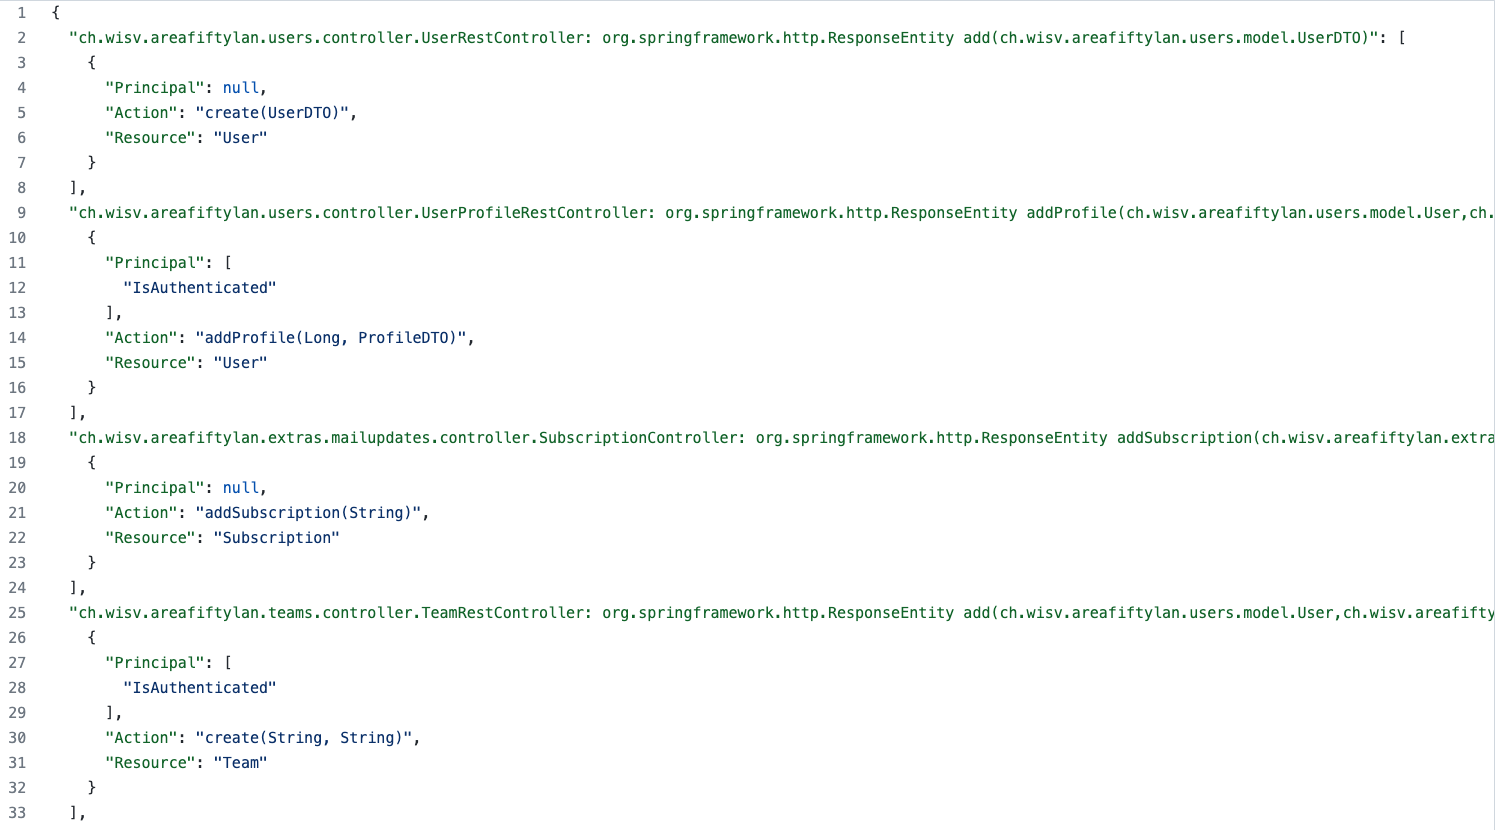
\includegraphics[width=0.45\textwidth]{img/policies.png}
%   \caption{polices}
%   \label{fig:policies}
% \end{figure}

